Resumen de las principales características de las variables relevantes en los registros de logs de navegación. Análisis de la distribución de los datos, incluyendo medidas de centralidad y dispersión. Usando la librería Pandas de Python, podemos obtener información importante sobre los conjuntos de datos. Estos valores nos proporcionarán un mayor entendimiento de la composición y estructura de los registros de navegación.

Podemos obtener información respecto a la cantidad de valores faltantes en el dataframe que se está utilizando, los cuales suman 36853 en total. De estos datos faltantes, 36853 corresponden principalmente al campo 'canal', con solo un valor faltante en el campo 'método'. Como se vio en el capítulo anterior, estos valores fueron eliminados del dataframe.

Haciendo uso de la misma librería, podemos determinar los tipos de datos que contiene cada campo:

\begin{itemize}
    \item \textbf{rut cliente:} Contiene datos de tipo int64.
    \item \textbf{fecha evento:} Contiene datos de tipo object.
    \item \textbf{metodo:} Contiene datos de tipo object.
    \item \textbf{canal:} Contiene datos de tipo object.
\end{itemize}

Además se puede conocer la cantidad de valores únicos que posee cada una de las columnas del dataframe (luego del proceso ETL):

\begin{itemize}
    \item \textbf{rut cliente:} Contiene 35541 valores únicos.
    \item \textbf{fecha evento:} Contiene 403259 valores únicos.
    \item \textbf{metodo:} Contiene 86 valores únicos.
    \item \textbf{canal:} Contiene 4 valores únicos.
\end{itemize}

La frecuencia con la que aparece cada canal es de:
\begin{itemize}
    \item PWA: 1437762
    \item WEB: 841642
    \item WEB-Actualizacion-datos: 12433
    \item WEB-Contacto-tramite-pension: 2335
\end{itemize}

Ahora se muestra un gráfico sobre la distribución de los canales en el conjunto de datos.

\begin{figure}[H]
    \begin{minipage}[t]{0.9\textwidth}
        \caption{Distribución de canales.}
        \label{descripcion_dataframe}        
    \end{minipage}

    \vspace{10pt}

    \begin{minipage}[b]{0.85\textwidth}
        \centering
        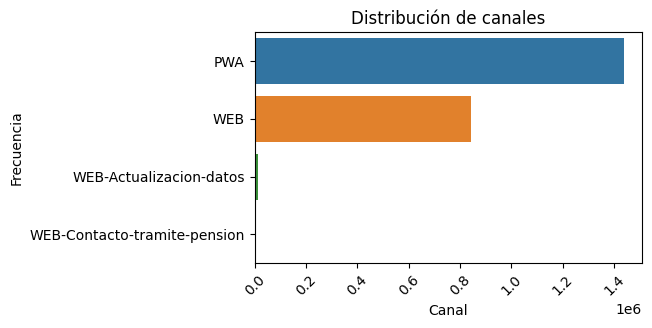
\includegraphics[width=\textwidth]{img/visualizacion-canales.png}        
    \end{minipage}

    \begin{minipage}[t]{0.9\textwidth}
        Fuente: Elaboración propia.
    \end{minipage}
\end{figure}

En la imagen se puede observar que principalmente dos canales predominan en cuanto a su frecuencia: PWA y WEB. Esto indica que actualmente los afiliados que utilizan la plataforma web tienden a utilizar estos dos canales, y en menor medida, los canales WEB-Actualización-datos y WEB-Contacto-tramite-pensión.

Para analizar las fechas, se decidió realizar una descripción de estas por día y hora. Año y mes quedan fuera del análisis ya que todos los datos pertenecen al mismo año y mes. Respecto a los días, en el set de datos hay un total de ocho días, y están presentes las veinticuatro horas del día. Estas tienen una frecuencia de:

\textbf{Distribución de días:}
\begin{itemize}
    \item 14: 4689
    \item 13: 4598
    \item 15: 4026
    \item 16: 2991
    \item 17: 2619
    \item 18: 1877
    \item 19: 211
    \item 20: 138
\end{itemize}

\textbf{Distribución de horas:}
\begin{itemize}
    \item 14: 1382
    \item 15: 1263
    \item 13: 1240
    \item 16: 1123
    \item 22: 1055
    \item 19: 1042
    \item 18: 1037
    \item 21: 1022
    \item 3: 1009
    \item 12: 999
    \item 23: 992
    \item 20: 985
    \item 17: 921
    \item 00: 890
    \item 1: 859
    \item 2: 800
    \item 4: 787
    \item 11: 726
    \item 10: 605
    \item 9: 540
    \item 8: 514
    \item 6: 463
    \item 7: 457
    \item 5: 438
\end{itemize}

Al analizar la distribución de los días, se observa que los días 14 y 13 presentan la mayor frecuencia en los registros, con 4689 y 4598 eventos, respectivamente. A medida que avanzan los días, se nota una disminución significativa en la cantidad de registros, llegando a solo 138 eventos el día 20.

En cuanto a la distribución de las horas, se puede observar que las horas 14, 15 y 13 tienen las frecuencias más altas, con 1382, 1263 y 1240 eventos, respectivamente. Las horas entre las 16 y las 21 también muestran una frecuencia considerablemente alta, mientras que las horas más tempranas (de 00 a 04) y las horas de la madrugada (después de las 04) presentan menor actividad, siendo la hora 05 la menos frecuente con 438 eventos.

Este análisis detallado por días y horas proporciona una visión más completa sobre la distribución temporal de los eventos registrados en el conjunto de datos, lo que puede ser útil para comprender los patrones de comportamiento de los usuarios en la plataforma.

Debido a la cantidad de datos únicos que presentan los otros campos se decidió evaluar otra forma de entregar esa información en la entrega final ya que resulta complejo añadirlo al informe sin que altere la visualización del resto de los datos del informe.